Da  die  Plots   wie  erw\"ahnt  den  Hauptteil   dieses  Berichts  ausmachen,
sind  die  meisten Informationen  und  Schlussfolgerungen  bereits im  Kapitel
\emph{Auswertung} zu finden.

Es  folgen hier  noch  eine Zusammenfassung  der  ermittelten Leitwerte  sowie
einige Anmerkungen zum Versuch allgemein.


% ---------------------------------------------------------------------------- %
\subsection{Resultate Leitf\"ahigkeit}
\label{sec:results:subsec:sigma}
% ---------------------------------------------------------------------------- %

F\"ur das Material des  Aluminium-Vollzylinders wurde folgende Leitf\"ahigkeit
ermittelt:

\begin{equation}
    \sigma_{Alu}
        = \overline{\sigma}_{Alu} \pm s_{\overline{\sigma}_{Alu}}
        = \SI[separate-uncertainty = true]{21.0 \pm 0.9 }{\mega\ampere\per\volt\per\meter}
        %= \SI[separate-uncertainty = true]{21031250.0 \pm 856224.181049733 }{\ampere\per\volt\per\meter}
\end{equation}


Wie  man  erkennen   kann,  weicht  dieser  Wert  doch   recht  bedeutend  vom
Literaturwert ab.:

\vspace{0.2em}
\begin{center}
    
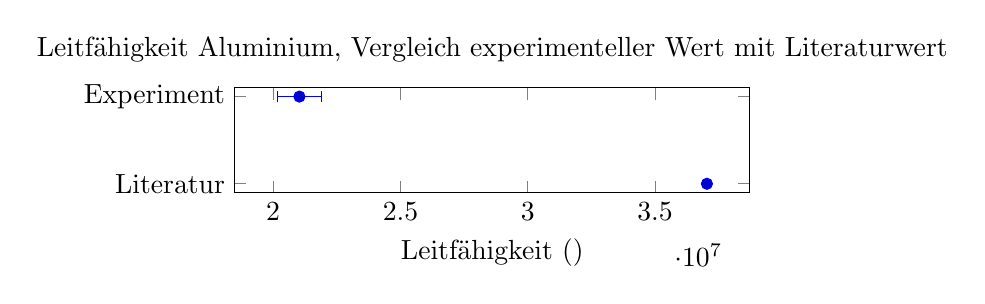
\begin{tikzpicture}
    \begin{axis}[
        try min ticks=2,
        width=.67\textwidth,
        height=.24\textwidth,
        title = {Leitf\"ahigkeit Aluminium, Vergleich experimenteller Wert mit Literaturwert},
        xlabel = {Leitf\"ahigkeit ($\si{\ampere\per\volt\per\meter}$)},
        symbolic y coords = {Literatur,Experiment}
    ]
    \addplot+[
        only marks,error bars/.cd,
        x dir=both,x explicit,
        error bar style={line width=0.5pt},
        ]
    coordinates {%
        (37037037.03703704,Literatur)
        (21031250.0,Experiment) +- (856224.181049733,0)
    };
    \end{axis}
\end{tikzpicture}
\captionof{figure}{%
    Vergleich  der experimentell  bestimmten  Leitf\"ahigkeit f\"ur  Aluminium
    mit  dem   Literaturwert  aus   Kuchlings  \emph{Taschebuch   der  Physik}
    \cite{ref:kuchling:resistivityTable}%
    }

\end{center}
\vspace{0.2em}

Beim Hohlzylinder aus  Kupfer waren der experimentell ermittelte  Wert und der
Literaturwert  doch  einiges n\"aher  zusammen,  auch  wenn das  Resultat  des
Experiments doch ein wenig kleiner ist als der Literaturwert:


\begin{equation}
    \sigma_{Cu}
        = \overline{\sigma}_{Cu} \pm s_{\overline{\sigma}_{Cu}}
        = \SI[separate-uncertainty = true]{52.8 \pm 0.2 }{\ampere\per\volt\per\meter}
       % = \SI[separate-uncertainty = true]{52800000.0 \pm 200006.624890277 }{\ampere\per\volt\per\meter}
\end{equation}

\begin{center}
    
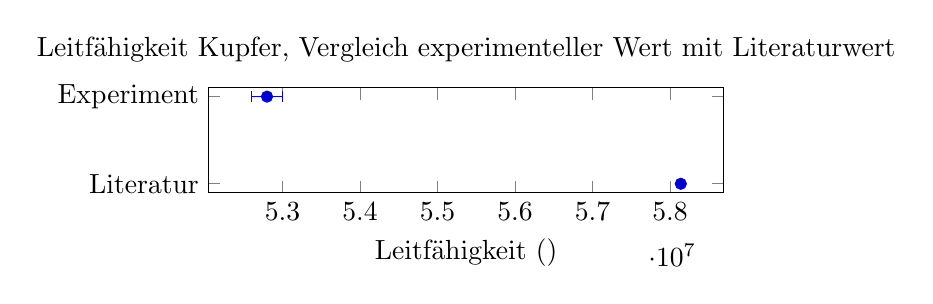
\begin{tikzpicture}
    \begin{axis}[
        try min ticks=2,
        width=.67\textwidth,
        height=.24\textwidth,
        title = {Leitf\"ahigkeit Kupfer, Vergleich experimenteller Wert mit Literaturwert},
        xlabel = {Leitf\"ahigkeit ($\si{\ampere\per\volt\per\meter}$)},
        symbolic y coords = {Literatur,Experiment}
    ]
    \addplot+[
        only marks,error bars/.cd,
        x dir=both,x explicit,
        error bar style={line width=0.5pt},
        ]
    coordinates {%
        (58139534.883720934,Literatur)
        (52800000.0,Experiment) +- (200006.624890277,0)
    };
    \end{axis}
\end{tikzpicture}
\captionof{figure}{%
    Vergleich  der  experimentell   bestimmten  Leitf\"ahigkeit  f\"ur  Kupfer
    mit  dem   Literaturwert  aus   Kuchlings  \emph{Taschebuch   der  Physik}
    \cite{ref:kuchling:resistivityTable}%
    }

\end{center}

Auch  beim  rostfreien  Stahl  liegen  das  Resultat  des  Versuches  und  der
Referenzwert nicht allzu weit auseinander. Wie  bereits bei der Auswertung und
in Anhang  \ref{app:steel} erl\"autert, wurden f\"ur  den Referenzwert Angaben
aus verschiedenen Quellen miteinander verrechnet.

\begin{equation}
    \sigma_{St}
        = \overline{\sigma}_{St} \pm s_{\overline{\sigma}_{St}}
        = \SI[separate-uncertainty = true]{1.19 \pm 0.03 }{\ampere\per\volt\per\meter}
        %= \SI[separate-uncertainty = true]{1190000.0 \pm 28108.0504482257 }{\ampere\per\volt\per\meter}
\end{equation}


\vspace{0.2em}
\begin{center}
    
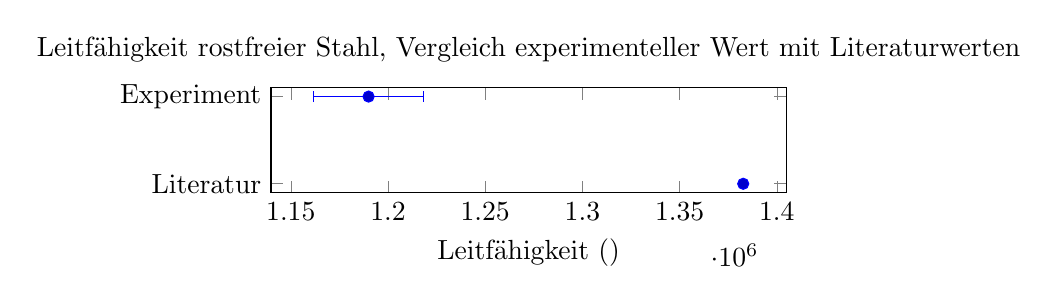
\begin{tikzpicture}
    \begin{axis}[
        try min ticks=2,
        width=.67\textwidth,
        height=.24\textwidth,
        title = {Leitf\"ahigkeit rostfreier Stahl, Vergleich experimenteller Wert mit Literaturwerten},
        xlabel = {Leitf\"ahigkeit ($\si{\ampere\per\volt\per\meter}$)},
        symbolic y coords = {Literatur,Experiment}
    ]
    \addplot+[
        only marks,error bars/.cd,
        x dir=both,x explicit,
        error bar style={line width=0.5pt},
        ]
    coordinates {%
        (1382711.1306243965,Literatur)
        (1190000.0,Experiment) +- (28108.0504482257,0)
    };
    \end{axis}
\end{tikzpicture}
\captionof{figure}{%
    Vergleich  der experimentell  bestimmten Leitf\"ahigkeit  f\"ur rostfreien
    Stahl  mit  einem  aus   Literaturwerten  bestimmten  Wert  (siehe  Anhang
    \ref{app:steel})%
    }

\end{center}
\vspace{0.2em}

Man kann also erkennen, dass Leitwerte  aus Tabellen mit Vorsicht zu geniessen
sind, und dass die effektiven  Leitwerte teilweise bedeutend kleiner ausfallen
k\"onnen als in der Literatur angegeben.


% ---------------------------------------------------------------------------- %
\subsection{Was man noch machen k\"onnte}
\label{sec:results:subsec:whatnext}
% ---------------------------------------------------------------------------- %

Den  Autor  reizt  es  zugegebenermassen   stark,  das  Fitten  in  Python  zu
automatisieren,  anstatt von  Hand  auszuf\"uhren. Leider hat  aber auch  sein
Arbeitstag lediglich  24 Stunden  plus die Nacht,  womit ein  solches Vorhaben
zumindest vorerst eine Tr\"aumerei bleiben muss.


Weiter  k\"onnte  man noch  den  mathematischen  Feinheiten nachgehen,  welche
hinter   den    in   Abschnitten   \ref{sec:ausw:subsec:hohlz:cu:subsubsec:LR}
ab     Seite    \pageref{sec:ausw:subsec:hohlz:cu:subsubsec:LR}     respektive
in    Abschnitt     \ref{sec:ausw:subsec:hohlz:st:subsubsec:LR}    ab    Seite
\pageref{sec:ausw:subsec:hohlz:st:subsubsec:LR}    beobachteten   Abweichungen
zwischen  den N\"aherungen  f\"ur  numerische Problemf\"alle  und den  exakten
L\"osungen stehen.


% ---------------------------------------------------------------------------- %
\clearpage
\subsection{Pers\"onliches Fazit}
\label{sec:results:subsec:thoughts}
% ---------------------------------------------------------------------------- %


Wie am  Umfang dieses  Berichts zu  erkennen ist, ist  der Autor  diesem Thema
gegen\"uber sehr interessiert eingestellt, und alles in Allem hat diese Arbeit
Spass gemacht.


Ein  kleiner  Verbesserungsvorschlag  sei   an  dieser  Stelle  trotzdem  noch
gemacht: Besonders in  der Vorbereitung  hatte der  Autor zeitweise  ein wenig
M\"uhge, den ``roten Faden'' der  ganzen Geschichte zu sehen (welche Messungen
sind durchzuf\"uhren,  welche sind nicht durchzuf\"uhren,  welche Auswertungen
sind zu machen, welche nicht). Vielleicht k\"onnte hier eine kurze \"Ubersicht
im Sinne  einer TODO-Liste in  der Versuchsanleitung Abhilfe  schaffen, anhand
derer man auf einen Blick erkennen kann, was zu tun ist, was nicht, und wo man
mit seiner Arbeit steht.


Im Grossen und Ganzen aber wie  gesagt ein interessanter Versuch, der gefallen
hat.
